\chapter{Exploratory data analysis}
During the previous chapter, we saved a clean and organized dataset. In this chapter we process the cleaned dataset to make it ready for immediate use for machine learning model training. We perform the following list of tasks get a machine learning ready dataset. 
\begin{itemize}
    \item  Remove features that do not have predictive value
    \item Transform categorical features to numerical features
    \item Select dependent and independent features 
    \item Split dataset into training and testing parts
\end{itemize}

\section{Select features relevant to customers}
In this project our objective is to predict response of customers to future telemarketing campaign given a given set of customer information, features related to the campaign and other features not related directly to the customers themselves should be excluded when developing our predictive machine learning model. In our dataset, the feature relevant to the customers are the demographics (age,job,marital,education) and cucstomer financial data (default,balance,housing,loan). Only these 8 features and the response (target) variable should be considered when we develop our model. 

\section{Transform categorical features into numerical features}
Machine learning algorithms do not work with categorical features. Only features with numberical values are employed by all machine learning algorithms. Hence, categorical features have to be transformed to numbers. As shown above our dataset consists of 7 categorical features. For example the feature \hl{education} consisted of text labels {\color{blue} tertiary, secondary, primary, unknown}. One may map the numbers 1, 2, 3, ,4 to each of the text labels of the feature and thereby transform the categorical feature to numerical feature called {\color{blue} \textbf{ordinal feature}}. At first, this kind of mapping may seem to make some sense with 1 corresponding to the highest educational level and 4 to the lowest level. Nevertheless, when in employed in a machine learning model it will be treated just like any other numerical. Specifically, for models that seek to find a linear relationship between features and response the encoding might might lead to undesirable effect. Depending on how linear the relationship of the features and the response variable, such ordinal encoding might work well or not. Nevertheless, the limitation imposed by ordinal transformation could be avoided by the use of another versatile and popular method of categorical encoding called one-hot encoding (OHE).

One-hot encoding (OHE) is a way to encode categorical features without intoducing unintended feature/response relationships like an ordinal encoding, by expanding the categorical feature into as many new features as the number of distinct feature values. For example, in our case OHE will split the feature \hl{education} into 4 columns corresponding to the number of text labels. Every row will have a value equal to '1' in exactly one column and a '0' elsewhere.

In figure \ref{fig:df_OHE} a preview of one hot encoded of our dataset is shown.
 
\begin{figure}[tbh]
\centering
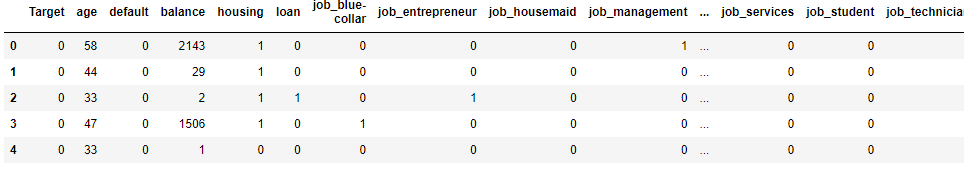
\includegraphics[width = 1.0\hsize]{./resources/img/fig_df_OHE.png}
\caption{Preview of our dataset where categorical features are transformed into numerical features with mapping and OHE.} 
\label{fig:df_OHE}
\end{figure}

It must be noted that in the case of a categorical feature with at most 2 unique values, the use of of ordinal encoding is justified as two points always define a straight line. Hence, any model including a model that seeks a linear relationship should work well.

\section{Feature selection and Train/test split}

The first column named \hl{Target} represent the outcome of the campaign and is selected as our independent feature while remaining 21 columns, which contain customer information are selected as dependent features.Also, in order to assess the predictive power of machine learning models it is important to split the data before training the model. The data split labeled as train is used to train the model, while the test split is reserved to assess the performance of the developed model. We split our dataset with train/test ratio of 80:20.






